你成功营救出了维火女，你们一同回到大陆中，继续冒险。她手中正是那樱花之泪。
\section{最小生成树}
王国的指挥官们解决了最短路径问题之后，又提出了一个新的问题：目前据点之间通信只能通过信使传递，他们希望在据点之间铺设通信线缆，使得信息可以顺着线缆迅速传递。
指挥官们认为，没有必要在任意两个据点之间都铺设线缆，而是只要能够保证任意两个据点之间都可以通过线缆连通即可。
这样一来，即使信息需要经过其他据点中转，也能实现整个王国的线缆通信。

然而，铺设线缆需要耗费大量资源。不同据点之间铺设线缆所需的成本各不相同。指挥官们希望找到一种方案：既能保证所有据点都连通，又能使铺设线缆的总成本尽可能低。
应该如何设计这样的方案呢？这其实就是\term{最小生成树}的问题：


给定一个\uline{连通的}无向带权图 \(G=(V,E)\)，如果从图中选择若干条边，使得所有顶点连通且不存在环，
那么图的所有顶点及这些边构成的子图就是原图的一棵\term{生成树}。在所有生成树中，边权总和最小的生成树称为\term{最小生成树（Minimum Spanning Tree，MST）}。\\

对此问题，格佛莱指出：初始时随意选择一个顶点s，然后选择依附于s的边权最小的一条边，将该边与相连顶点“收进来”，
此时，当前的生成树中就已经有了2个顶点。然后，继续选择能够连通这2个顶点与其他顶点的一条边权最小的边，并将该边与相连的顶点“收进来”，生成树中就有了3
个顶点。重复这个操作，直至所有顶点都被“收进来”。这样做，得到的生成树中的所有边，一定是使得顶点连通的所有边的选集中权值之和最小的$N-1$条边。
如图\ref{fig:Prim算法道理说明}所示，使得三个顶点连通，可选的边集有$\{e_0, e_1\}$、$\{e_0, e_2\}$以及$\{e_1, e_2\}$，权值之和最小的一定是$\{e_0, e_1\}$。

因此得到的树一定就是最小生成树。这就是\term{Prim（普里姆）算法}的核心思想。
\begin{figure}[htbp]
    \centering
    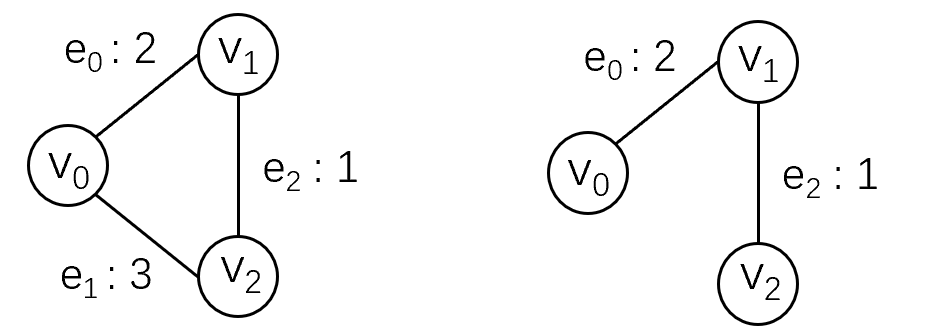
\includegraphics[width=0.50\textwidth]{assets/pics_and_ppts/ch5/24Prim算法道理说明.png}
    \caption{}
    \label{fig:Prim算法道理说明}
\end{figure}

可以看出，对于Prim算法，我们需要动态维护当前生成树以及尚未收入的所有顶点到当前生成树的最小代价。详细实现如下。
\subsection{Prim（普里姆）算法}
设无向连通图$G=(V,E)$，Prim算法的过程如下：设置集合S保存已经收入当前的生成树中的顶点，cur\_mind[]保存各未收入顶点到集合S的最小代价。
初始时随意收入一个顶点s（即S=\{s\}），令与s邻接的所有顶点的cur\_mind[]为相应边权，令其他所有顶点的cur\_mind[]为正无穷。然后执行$N-1$次以下两个步骤：
\begin{enumerate}
    \item 从集合V-S（还未收入当前生成树的顶点集）中选择距离集合S代价最小的一个顶点（即cur\_mind[]最小）u，将u加入S，并将u以及这条边加入当前生成树中。
    \item 对于 u 的每个未被收入S的邻接点 v，执行 
    \[
        cur\_mind[v] = min(cur\_mind[v], cost(u, v))
    \] 
    即如果通过 u 到达 v 的代价比原来记录的更小，则更新 cur\_mind[v]。
\end{enumerate}
可以看到这个过程与迪杰斯特拉算法非常像，迪杰斯特拉算法是每次选择与\uline{源点s}最近的顶点，而Prim算法是选择与\uline{已有生成树S}最近的顶点。注意：Prim算法中，
cur\_mind[v]记录的并不是顶点v到源点s的最短距离，而是顶点v到集合S的最短距离，即v到S中的所有顶点的距离中最小的那个。

我们以图\ref{fig:Prim算法过程演示} a）所示的图，演示一遍Prim算法的过程：

1）任选一个点，假设选A，收入最小生成树，更新A的邻接点B和C的cur\_mind[]，如b）所示；此时集合S为\{A\}。图中带下划线的数字表示还未收入生成树的各个顶点
距集合S的最小代价（最短距离）；图中虚线表示该顶点最近是被哪条边所更新的，收入该顶点时沿着虚线就能找到边。

\begin{figure}[htbp]
    \centering
    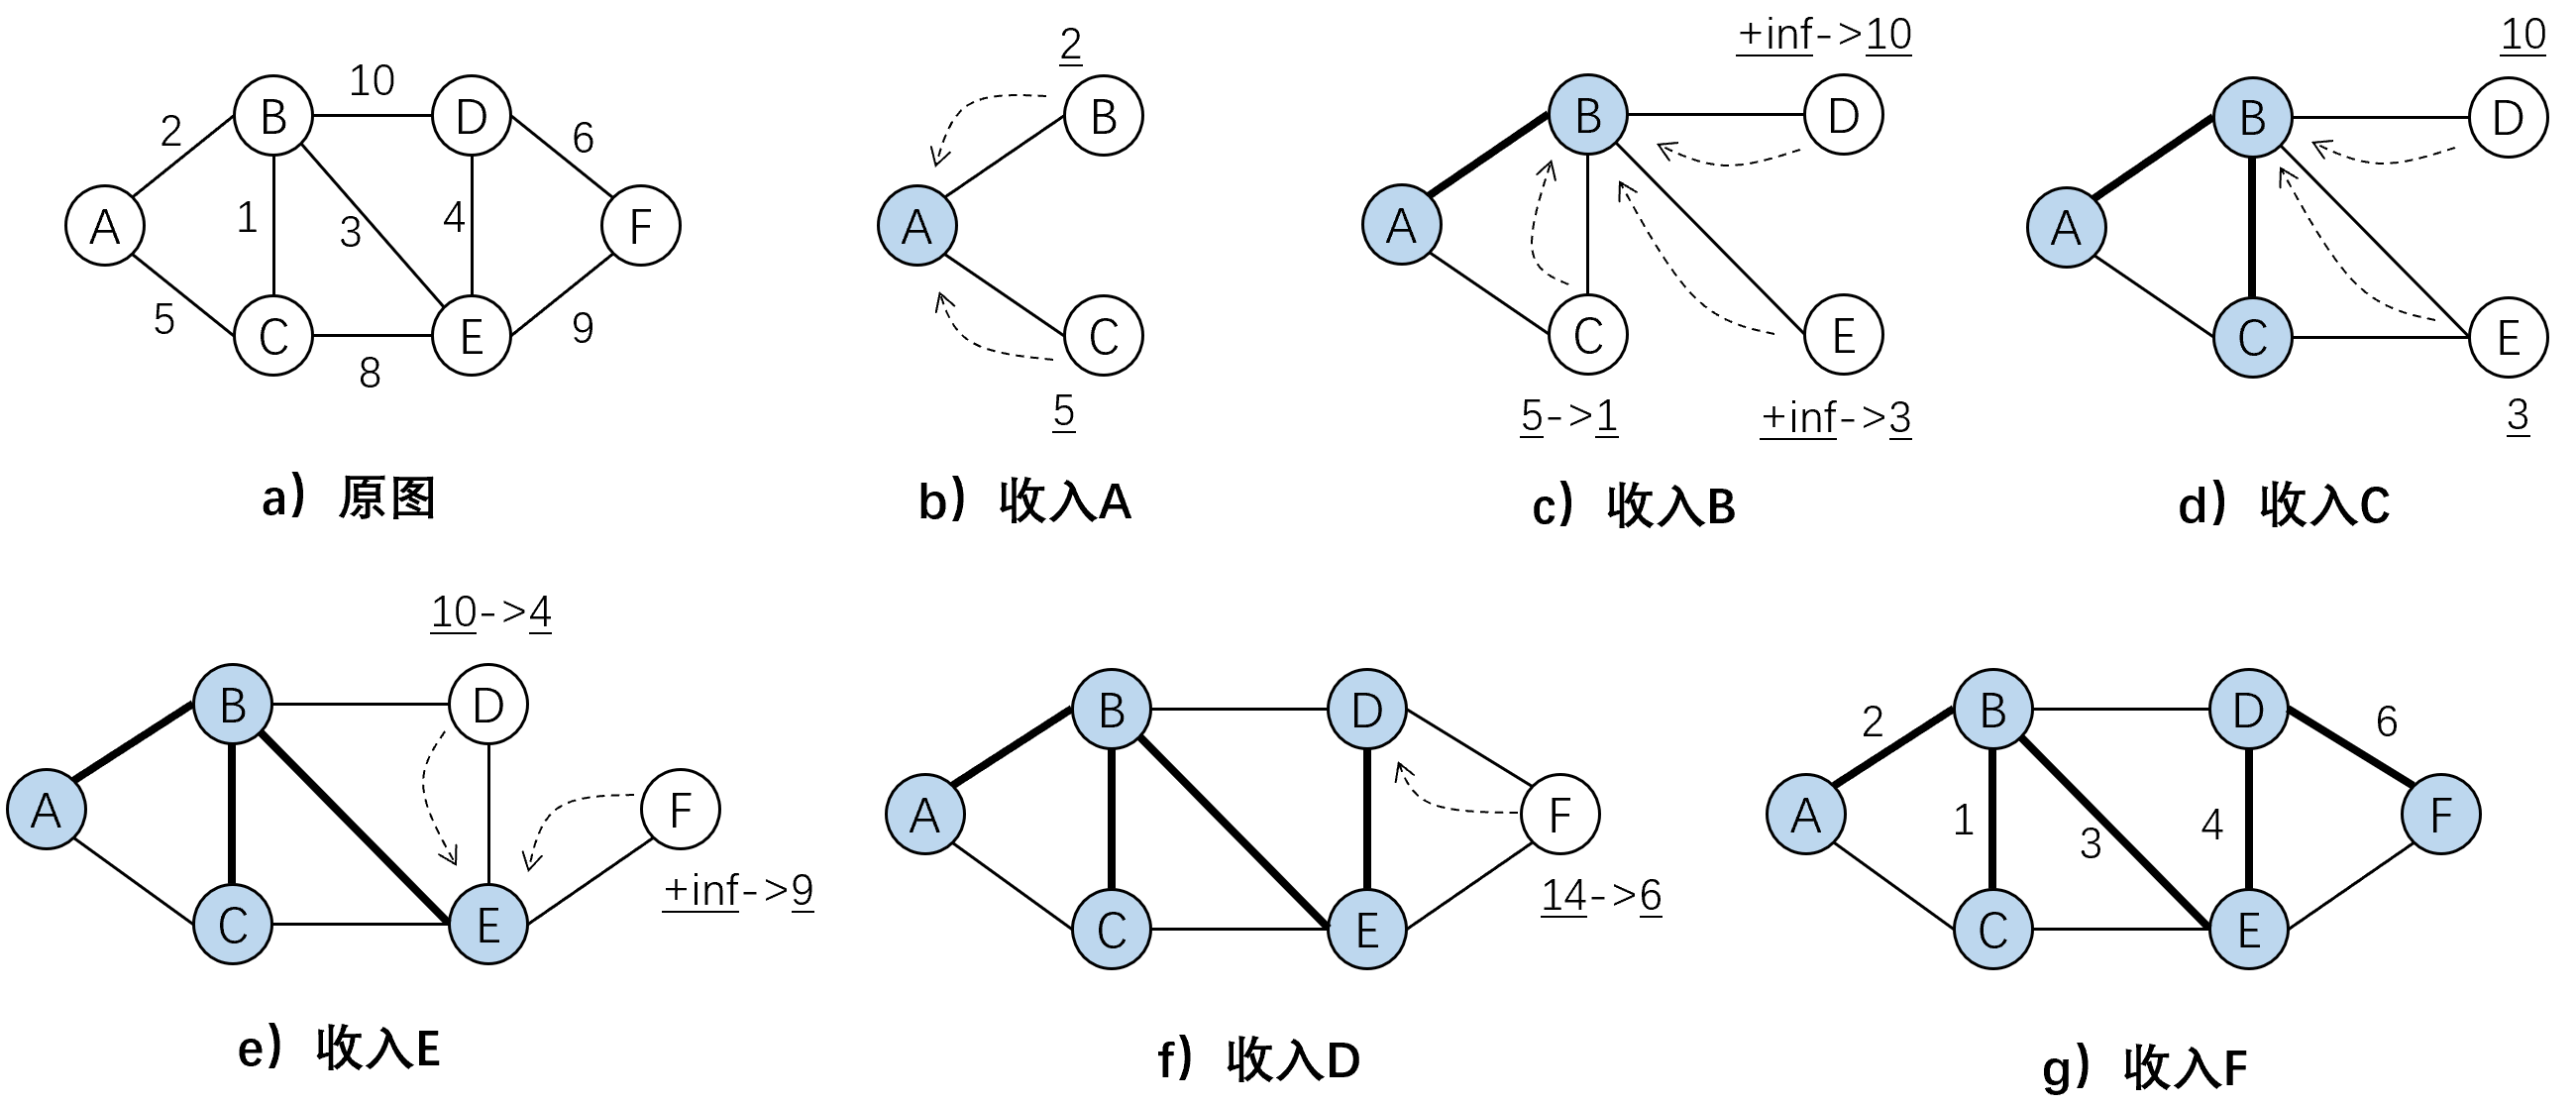
\includegraphics[width=1.01\textwidth]{assets/pics_and_ppts/ch5/25Prim算法过程演示.png}
    \caption{Prim算法过程演示}
    \label{fig:Prim算法过程演示}
\end{figure}

2）未收入的顶点中，到集合S代价最小（最近）的顶点是B，于是收入B，如c）所示，收入B后，
由于 $cur\_mind[C] = 5 < cost(B, C) = 1$，也就是说对于新的集合S=\{A, B\}，C到B的距离更小了，于是更新C到集合S的距离为1。类似地，更新cur\_mind[E]为3、
cur\_mind[D]为10。

3）未收入的顶点中，到集合S代价最小（最近）的顶点是C，于是收入C，如d）所示，并且对于C的邻接点E，由于$cur\_mind[E] = 3 < cost(C, E) = 8$，因此无需更新。

4）收入E，然后更新D、F，如e）所示；

5）收入D，然后更新F，如f）所示；

6）收入F，所有顶点均已被收入生成树，此时得到的即是最小生成树，各个边的权值之和即是最小代价：2 + 1 + 3 + 4 + 6 = 16。\\



\subsection{Kruskal（克鲁斯卡尔）算法}
\label{subsec:Kruskal算法}
指挥官麦丽凯给出了一种完全不同的思路：她不喜欢一步一步细致、缜密地规划，而是将注意力放眼全局。
麦丽凯指出：初始时，没有任何顶点和边被收入生成树，将图看成是$N$个割裂的顶点构成了$N$个连通块。首先挑选整个图中边权最小的边，将它以及它连通的两个顶点
加入生成树，连通块的数量便还剩$N-1$个。此后，每次选择剩余边中权值最小的，若它所连接的两个顶点处在不同连通块，则将他们连通并收入生成树，直至所有顶点均已连通。

该策略显然是正确的。因为如果两个连通块之间存在一条权值最小的边，那么最优解是一定要包含这条边的。
这种放眼全局，通过不断地选择边权最小的边将不同连通块合并的策略，这就是\term{Kruskal（克鲁斯卡尔）算法}的核心思想。


具体来说，设无向连通图$G=(V,E)$有$N$个顶点，Kruskal算法的过程如下：
将图看成是$N$个割裂的顶点构成了$N$个连通块。然后反复按边权从小到大检查所有还未被收入生成树的边，
若被检查的边所连接的两个顶点不在同一个连通块中，则将他们连通，并收入生成树，否则跳过，继续检查下一条边。
如此重复，直至所有顶点均已连通；

我们以\ref{fig:Kruskal算法过程演示} a）所示的图演示一遍Kruskal算法的过程。

1）所有边中权值最小的是连接BC的边（为1），将其收入，如b）所示，此时B、C已被连通；

2）此时剩余所有边中，边权最小的是连接A、B的边（为2），由于A、B此时不在相同的连通块，因此将他们收入生成树，此时A、B、C已被连通，如c）所示；

\begin{figure}[htbp]
    \centering
    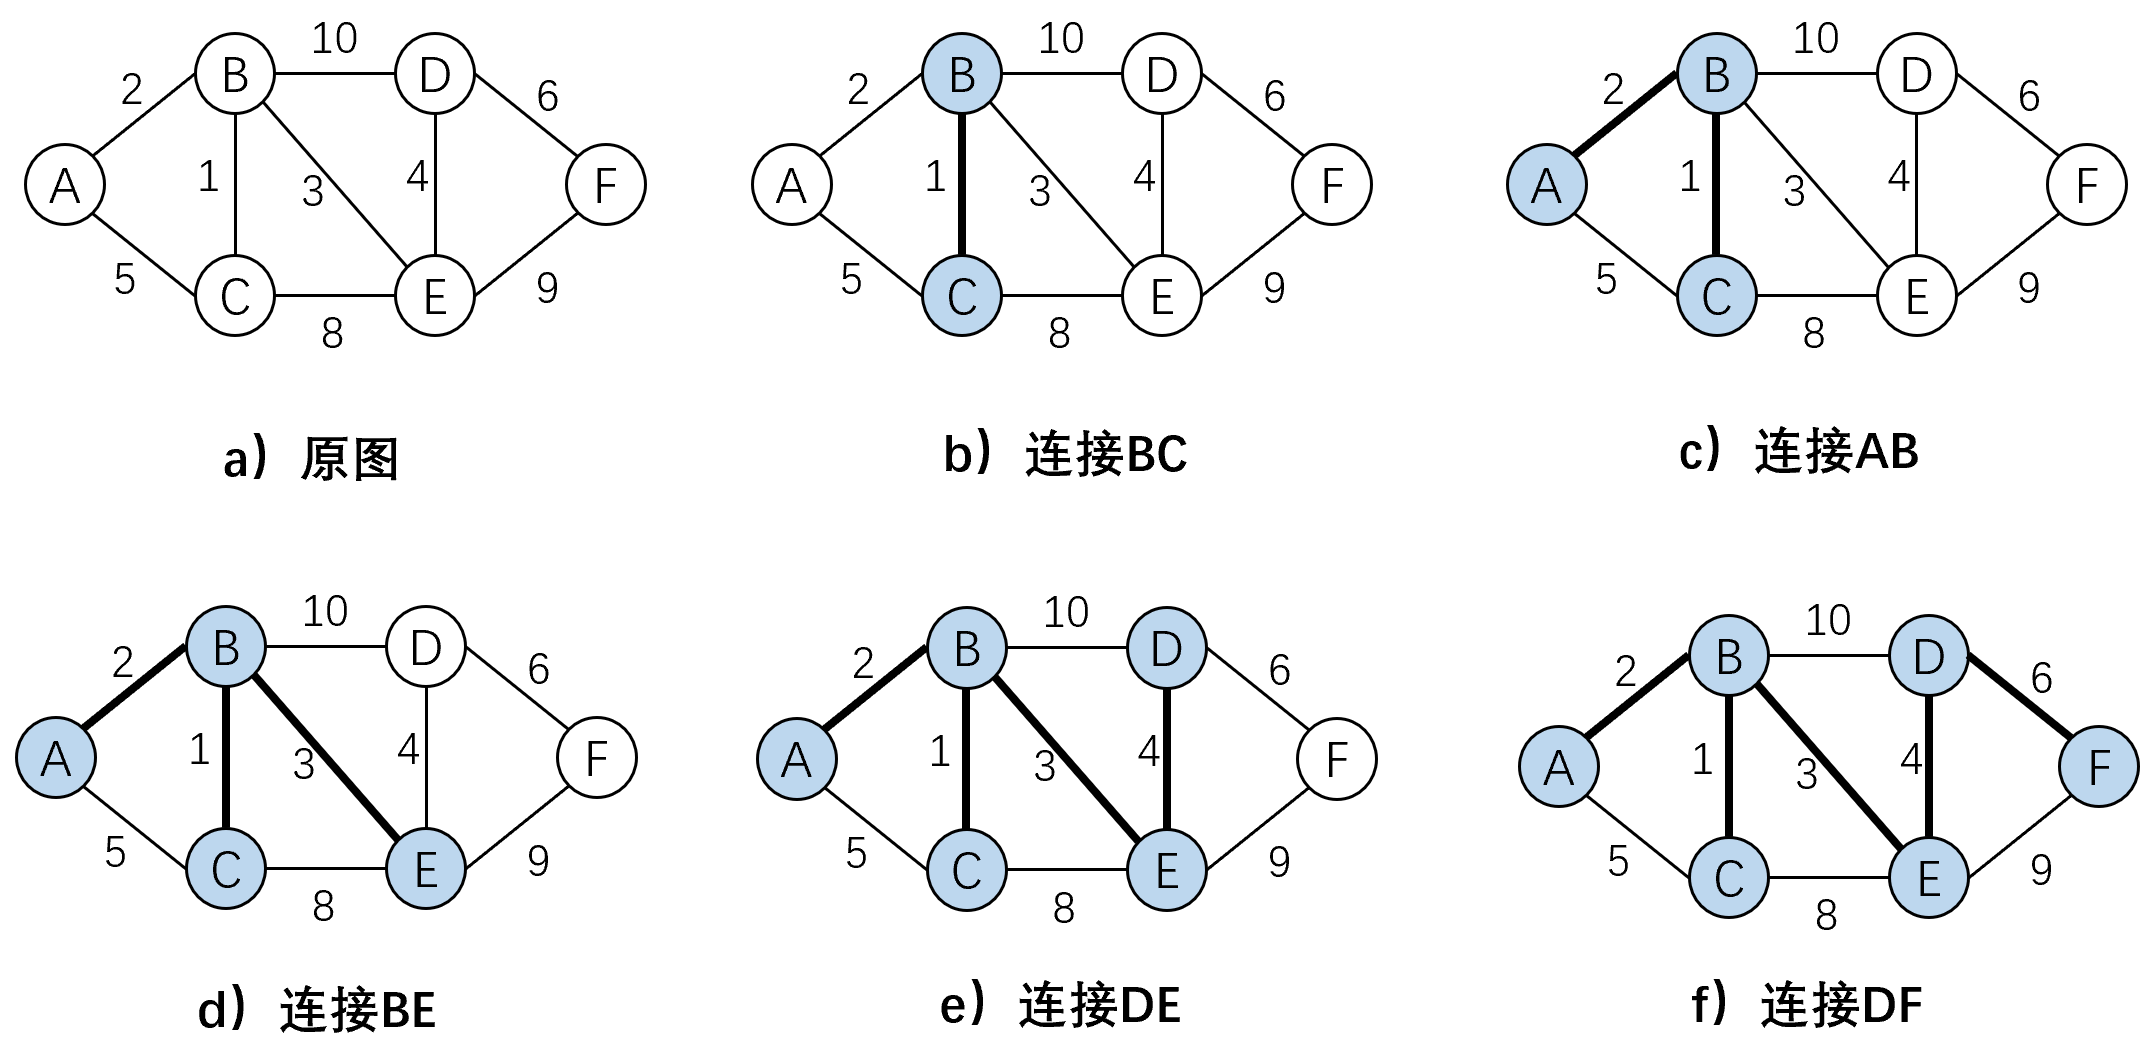
\includegraphics[width=0.95\textwidth]{assets/pics_and_ppts/ch5/26Kruskal算法过程演示.png}
    \caption{Kruskal算法过程演示}
    \label{fig:Kruskal算法过程演示}
\end{figure}

3）此时剩余所有边中，边权最小的是连接B、E的边（为3），由于B、E此时不在相同的连通块，因此将他们收入生成树，此时A、B、C、E已被连通，如d）所示；

4）将D收入生成树，此时A、B、C、E、D已被连通，如e）所示；

5）剩余所有边中，边权最小的是连接A、C的边（为5），但A、C已经处于同一个连通块，因此跳过，继续检查下一条边；

6）剩余所有边中，边权最小的是连接D、F的边（为6），并且D、F处在不同的连通块，于是将它们收入生成树，如f）所示，此时所有顶点均已被连通，算法结束。可以看到，
在这个图的例子中，Kruskal算法得到了与Prim算法相同的最小生成树。

\subsection{算法实现}
\minisection{Prim算法的实现}
Prim算法的代码与Dijkstra算法非常相似。以邻接表为例，Prim算法的实现如下所示（高亮部分是与Dijkstra的区别部分）：
\begin{cppcodeHighlight}[15,33,39-40]
    struct EdgeInfo {
        int u;
        int weight;
    };
    vector<EdgeInfo> AdjList[N];
    const int inf = 0x3fffffff;
    bool solved[N]; // 已初始化为false
    int cur_mind[N];    // 已初始化为inf
    int Pre[N];     // 已初始化为-1

    // 返回生成树的最小代价。
    int Prim(int s) {
        cur_mind[s] = 0;
        // min_cost用于累加生成树的最小代价，算法返回它
        int min_cost = 0;
        // 为了代码简洁，将收入s的操作放在循环里了，因此要做N次循环
        for(int i=0; i<N; i++) {
            int v = -1;
            int min_curmind = inf;
            for(int j=0; j<N; j++) {
                if(!solved[j] && cur_mind[j] < min_curmind) {
                    min_curmind = cur_mind[j];
                    v = j;
                }
            }

            // 图不连通
            if(v == -1) {
                return -1;
            }
            solved[v] = true;
            // 累加代价
            min_cost += cur_mind[v];
            
            for(int j=0; j<AdjList[v].size(); j++) {
                int u = AdjList[v][j].u;
                int weight = AdjList[v][j].weight;
                // 新加入集合的v，能使的u到集合的距离更小
                if(weight < cur_mind[u]) {
                    cur_mind[u] = weight;
                    Pre[u] = v;
                }
            }
        }
        return min_cost;
    }
\end{cppcodeHighlight}
若需要知道这棵最小生成树“长什么样”，则可以在每次选出顶点 v 时，打印出 Pre[v] 和 v，它们即构成了最小生成树中的一条边。同时可以看出，
与迪杰斯特拉算法类似，“选点”的过程同样可以通过堆优化。\\


\minisection{2.Kruskal算法实现}
Kruskal算法需要每次选择边权最小的边，若每次遍历邻接表或邻接矩阵进行“选边”，代价显然无法接受。因此，要实现Kruskal算法，通常需要将所有边按边权排序，
排好序后每次按顺序选择即可。这里为大家引入C++中的标准库sort函数。

\begin{cppcode}
    struct EdgeInfo {
        int u,v;
        int weight;
        // 定义两个EdgeInfo结构体的“<”比较规则
        bool operator < (const EdgeInfo& other) {
            return this->weight < other.weight;
        }
    };
    EdgeInfo edges[M];  // 假设已经存储了图G中所有边的信息
    
    
    int Kruskal() {
        // 按照EdgeInfo的“<”比较规则，对edges数组进行排序。
        std::sort(edges, edges+M);
        // ...
    }
\end{cppcode}

通过上面的代码，就将edges这个数组按照其元素weight的大小关系，排成了一个从小到大的有序数组。
关于结构体的比较规则定义、std::sort的使用请参见第\pageref{sec:为结构体定义比较规则、std::sort()的使用}页。



Kruskal算法选边时，需要判断两个顶点是否在同一个连通块中，若不在，需要将两个连通块合并，这正是并查集提供的功能！我们这里直接使用\ref{sec:并查集}节中提供的
并查集的Find与Union操作。若将所有边遍历一轮之后，收入生成树的边的数量不足$N-1$，说明图不连通。可以写出Kruskal的代码如下：
\begin{cppcode}
    int Kruskal() {
        // 按照EdgeInfo的“<”比较规则，对edges数组进行排序。
        std::sort(edges, edges+M);
        // 要返回的生成树最小代价
        int min_cost = 0;
        // 已收进来的边的数量
        int edgenum_in_tree = 0;
        int father[N];
        for(int i=0; i<N; i++) {
            father[i] = i;
        }

        // 遍历所有边
        for(int i=0; i<M; i++) {
            int u = edges[i].u;
            int v = edges[i].v;
            int u_id = Find(father, u);
            int v_id = Find(father, v);
            // 这条边连接的u、v不在同一个集合
            if(u_id != v_id) {
                Union(father, u, v);
                min_cost += edges[i].weight;
                // cout << “选择了一条边u->v”
                edgenum_in_tree += 1;
            }
        }
        /* 原图不连通，不存在包含所有顶点的生成树。*/
        if(edgenum_in_tree < N-1) {
            return -1;
        }
        return min_cost;
    }
\end{cppcode}

